\begin{frame}{Giao diện quản lý GitOps bằng ArgoCD}
\begin{figure}[H]
\centering
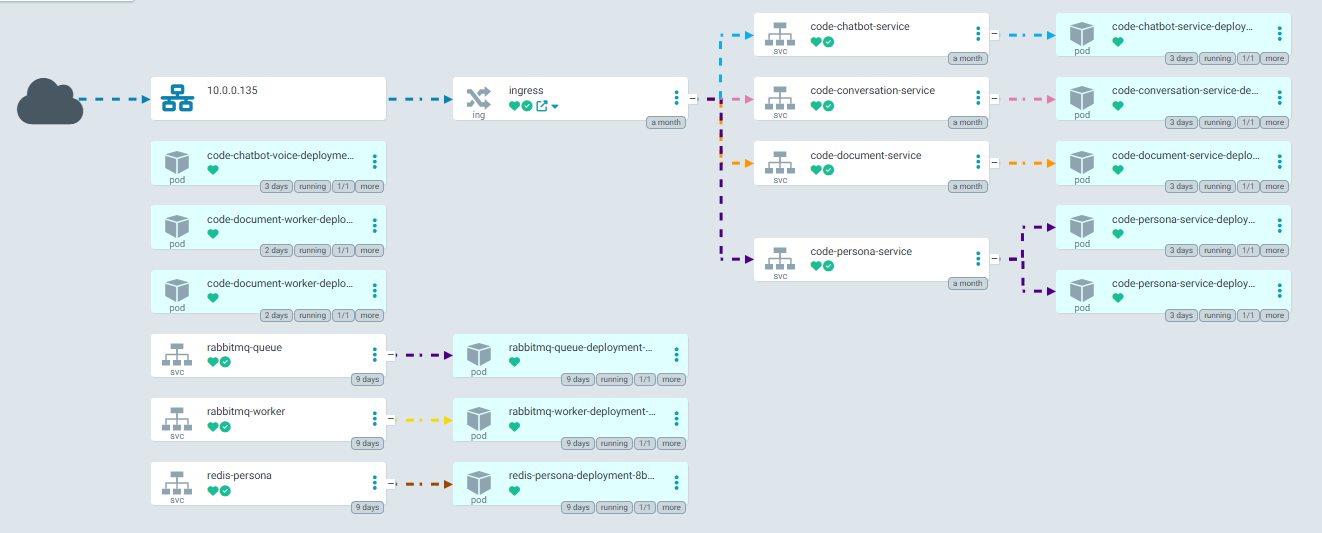
\includegraphics[height=0.55\textheight,width=0.9\textwidth,keepaspectratio]{pictures/argocd-web-ui.png}
\caption{Kết quả giao diện ArgoCD chạy docker trong kubernetes}
\end{figure}

\note{
ArgoCD được triển khai trong cụm Kubernetes để thực hiện quy trình Continuous Delivery (CD) theo mô hình GitOps.
ArgoCD liên tục giám sát kho lưu trữ Git chứa các file cấu hình Kubernetes. Khi phát hiện có sự thay đổi (ví dụ: phiên bản Docker image mới), ArgoCD sẽ tự động đồng bộ (sync) và cập nhật các Pod đang chạy trên Kubernetes thực tế để khớp với cấu hình được khai báo trên Git.
}
\end{frame}
